\documentclass[compress]{beamer}
\usepackage{ifthen,verbatim}

\title{First look at CRUZET \\ track-based CSC alignment}
\author{K\'aroly Banicz, Jim Pivarski$^*$, Alexei Safonov$^*$}
\institute{US-CMS, $^*$Texas A\&M University}
\date{18 June, 2008}

\newcommand{\isnote}{}
\xdefinecolor{lightyellow}{rgb}{1.,1.,0.25}
\xdefinecolor{darkblue}{rgb}{0.1,0.1,0.7}

%% Uncomment this to get annotations
%% \def\notes{\addtocounter{page}{-1}
%%            \renewcommand{\isnote}{*}
%% 	   \beamertemplateshadingbackground{lightyellow}{white}
%%            \begin{frame}
%%            \frametitle{Notes for the previous page (page \insertpagenumber)}
%%            \itemize}
%% \def\endnotes{\enditemize
%% 	      \end{frame}
%%               \beamertemplateshadingbackground{white}{white}
%%               \renewcommand{\isnote}{}}

%% Uncomment this to not get annotations
\def\notes{\comment}
\def\endnotes{\endcomment}

\setbeamertemplate{navigation symbols}{}
\setbeamertemplate{headline}{\mbox{ } \hfill
\begin{minipage}{5.5 cm}
\vspace{-0.75 cm} \small
\end{minipage} \hfill
\begin{minipage}{4.5 cm}
\vspace{-0.75 cm} \small
\begin{flushright}
\ifthenelse{\equal{\insertpagenumber}{1}}{}{Jim Pivarski \hspace{0.2 cm} \insertpagenumber\isnote/\pageref{numpages}}
\end{flushright}
\end{minipage}\mbox{\hspace{0.2 cm}}\includegraphics[height=1 cm]{../cmslogo} \hspace{0.1 cm} \includegraphics[height=1 cm]{../tamulogo} \hspace{0.01 cm} \vspace{-1.05 cm}}

\begin{document}
\frame{\titlepage}

%% \begin{notes}
%% \item This is the annotated version of my talk.
%% \item If you want the version that I am presenting, download the one
%% labeled ``slides'' on Indico (or just ignore these yellow pages).
%% \item The annotated version is provided for extra detail and a written
%% record of comments that I intend to make orally.
%% \item Yellow notes refer to the content on the {\it previous} page.
%% \item All other slides are identical for the two versions.
%% \end{notes}

\begin{frame}
\frametitle{``CSC-Overlaps'' procedure}

\begin{columns}
\column{0.8\linewidth}
\begin{itemize}\setlength{\itemsep}{0.2 cm}
\item Different track-based alignment procedure from the one we
propose for high-luminosity samples
\item CSC-Overlaps procedure: look for tracks (tracklets?) passing
through two CSC chambers in the same ring
\item Two modes:
\begin{itemize}
\item move all chambers until track fits are consistent
\item propagate alignment from a known measurement (SLM-measured
chambers) to the chambers in between
\end{itemize}
\end{itemize}

\column{0.2\linewidth}
\includegraphics[width=\linewidth]{overlap.png}
\end{columns}

\begin{itemize}\setlength{\itemsep}{0.2 cm}
\item Can be used
\begin{itemize}
\item without a working silicon tracker
\item without fully-reconstructed tracks (just segments)
\item without modification for $\vec{B}$=on and $\vec{B}$=off
\end{itemize}
\item Independent development effort, largely by Karoly Banicz
\end{itemize}
% \hspace{-0.83 cm} \textcolor{darkblue}{\Large How it works}
\end{frame}

\begin{frame}
\frametitle{Status of all-at-once fit}

\vspace{-0.3 cm}
\begin{columns}
\column{0.1\linewidth}
\textcolor{darkblue}{\Large Method:}

\column{0.8\linewidth}
\begin{center}
\includegraphics[width=0.8\linewidth]{even-odd.png}
\end{center}

\column{0.1\linewidth}
\mbox{ }
\end{columns}

\vfill
\hspace{-0.83 cm} \textcolor{darkblue}{\Large Problem with convergence}

\begin{columns}
\column{0.3\linewidth}
\includegraphics[width=1.5\linewidth]{beamhalo_APE_r0_t100000_Xf0mm_iter100.png}

\column{0.7\linewidth}
\begin{itemize}
\item Starting from a perfectly-aligned detector, global distortion grows (iteration 100 shown on left)
\item Due to the fact that HIP minimizes {\it mean} of residual
distribution, and this global distortion introduces symmetric
double-peaks which preserve the mean
\end{itemize}
\end{columns}
\end{frame}

\begin{frame}
\frametitle{Solution (Method 2)}

\begin{itemize}
\item Don't want left-residuals and right-residuals to balance
\item Make sure that each chamber sees only one kind of residual
\item Align evens and odds at the same time, using left-sides and right-sides differently:
\end{itemize}
\begin{center}
\includegraphics[width=0.7\linewidth]{fit_to_both.png}
\end{center}

\begin{itemize}
\item Implemented but untried (start with the same MC sample)
\end{itemize}
\end{frame}

\begin{frame}
\frametitle{CRUZET data}

\begin{itemize}
\item Track-based/hardware comparison possible in ME+4
\item CRUZET-I data available for skimming
\item Too few tracks in the (narrow) overlap regions
\item Tracking may be too restrictive, e.g.\ requiring coincidence between stations
\item Built tracks out of pairs of segments in neighboring chambers
\item Quality cuts: (a) only one pair allowed, (b) segment-pair must be fitable to a single line with $\chi^2/\mbox{ndf}$ $<$ 10
\end{itemize}

\begin{columns}
\column{0.5\linewidth}
\includegraphics[width=\linewidth]{wxresid_chamber_604029568.png}
\column{0.5\linewidth}
\includegraphics[width=\linewidth]{wxresid_chamber_604029568_chi2cut.png}
\end{columns}
\end{frame}

\begin{frame}
\frametitle{Closer look\ldots}

\begin{center}
\includegraphics[width=0.8\linewidth]{wxresid_chamber_604029568_chi2cut.png}
\end{center}

\small
Comments:
\begin{itemize}
\item This pair has a $\sim$1.3~mm relative misalignment
\item 1.23~mm or 1.48~mm?  Alignment algorithm uses the mean
\item This is the biggest mean--Gaussian fit discrepancy we could find
\end{itemize}
\end{frame}

\begin{frame}
\frametitle{The ME+4 landscape}
\small
\begin{itemize}
\item Even without a convergent procedure, we can propagate from one reference measurement and compare against another
\item CRUZET-I: two good SLM lines, no tracks in chambers 1 and 8 (PG comparison only: chamber targets 2--7, SLM endpoints 10--16)
\end{itemize}
\begin{center}
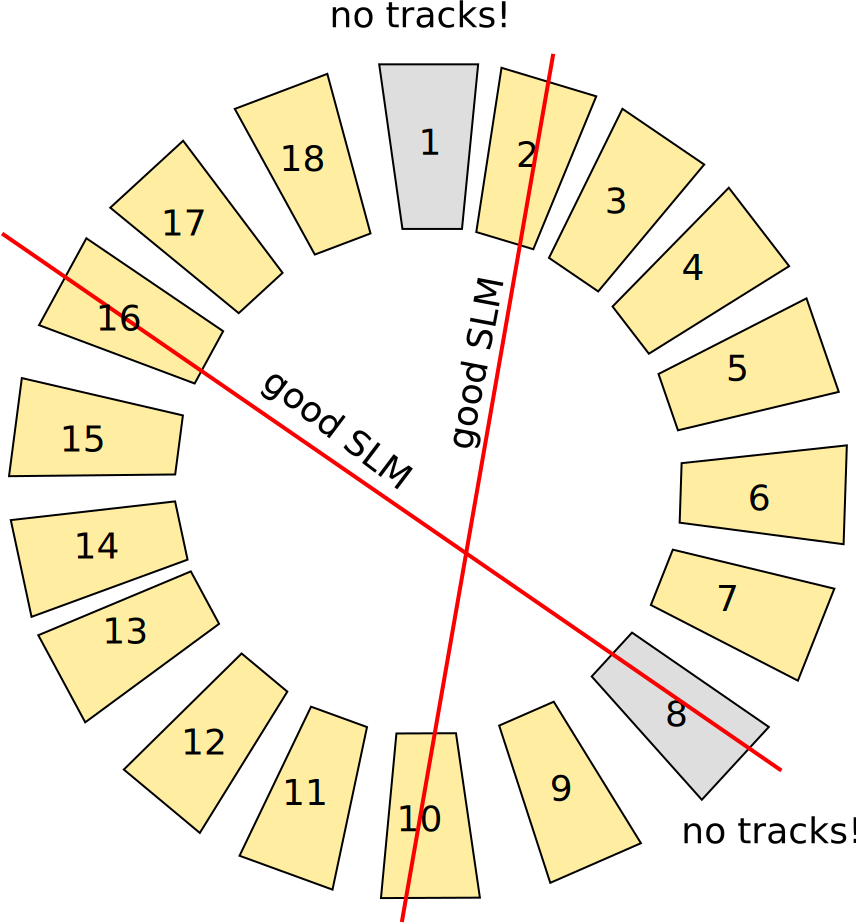
\includegraphics[width=0.4\linewidth]{landscape.png}
\end{center}
\begin{itemize}
\item CRUZET-II: all three SLM lines, unknown situation with tracks (maybe full comparison?)
\end{itemize}
\end{frame}

\begin{frame}
\frametitle{A more-basic PG test}

In addition, we can do a simple check against PG in all stations by 
\begin{itemize}
\item look at residuals with ideal geometry
\item look at residuals with PG geometry: should be closer to zero
\item doesn't depend on convergence of algorithm
\end{itemize}

\vspace{0.2 cm}
Oleg is filling an Excel spreadsheet that I can convert to an AlignmentRcd in the database

\vspace{0.2 cm}
We can attempt new global fit afterward on rings without empty chambers

\vfill
\hspace{-0.83 cm} \textcolor{darkblue}{\Large Inclusion of CRUZET-II}

\vspace{0.2 cm}
We should attempt a skim of the prompt RECO

\vspace{0.2 cm}
Maybe we can even merge track-based statistics?  ME+4 is not moved as often as the other disks (need to ask Armando)
\end{frame}

%% \section*{First section}
%% \begin{frame}
%% \begin{center}
%% \Huge \textcolor{blue}{First section}
%% \end{center}
%% \end{frame}

\begin{frame}
\frametitle{Summary status of CSC-Overlap}

\begin{itemize}\setlength{\itemsep}{0.3 cm}
\item Trigger issues (not discussed here) are basically solved
\item CSA08 MC event sample was very useful for vetting algorithm
\item No global convergence of an entire ring yet, but we understand what went wrong and have an idea to fix it
\item Residuals in data are usable, but full-ring fit is impossible if any chamber is missing or has low statistics
\item Basic comparison with PG possible in CRUZET-I
\item Comparison with PG+SLMs might be possible in CRUZET-II, depending on occupancy
\end{itemize}

\label{numpages}
\end{frame}

\end{document}
